\documentclass{article}
\usepackage[utf8]{inputenc}
\usepackage{graphicx}
\usepackage{subcaption}
\usepackage{amsmath}
\usepackage{tablefootnote}
\usepackage{csvsimple}
\usepackage{setspace}
\usepackage{amsthm}
\usepackage[ruled,vlined]{algorithm2e}
\usepackage{tikz}
\usetikzlibrary{arrows}
\usepackage[
  backend=biber,
  style=apa,
  citestyle=apa
]{biblatex}
\usepackage{geometry}
\geometry{
 a4paper,
 total={150mm,237mm},
 left=30mm,
 top=30mm,
 }
\newtheorem{definition}{Definition}
\newtheorem{remark}{Remark}
\newtheorem{corollary}{Corollary}
\newtheorem{theorem}{Theorem}
\def\indep{\perp \!\!\! \perp}
\def\notindep{\not\!\indep}
\renewcommand{\baselinestretch}{1.5} 
\addbibresource{references.bib}

\title{Causal Discovery of Macroeconomic DSGE Models}
\author{Emmet Hall-Hoffarth}
\date{\today}

\begin{document}

\maketitle

\abstract{This paper presents a set of criteria and an algorithm for agnostic, data-driven selection among macroeconomic DSGE models inspired by structure learning methods for DAGs. The state-space representation of any DSGE model is also a DAG, and therefore concepts used for model selection amongst DAGs can also be used in the context of DSGE models. This implies a set of criteria based on conditional independence tests which can be used to evaluate whether a state-space model, and thereby a DSGE model is consistent with some observed data. I then introduce an algorithm which tests these criteria against the set of possible state-space models producing a subset of allowable models. When combined with likelihood maximisation this algorithm identifies a unique optimal model. The efficacy of this alogorithm is demonstrated for simulated data, and results for real data are also provided and discussed.}

\section{Introduction}

\section{Liturature Review}

\subsection{DAGs} \label{dags}

\subsubsection{Preliminaries} \label{prelim}

\begin{figure}
  \centering
  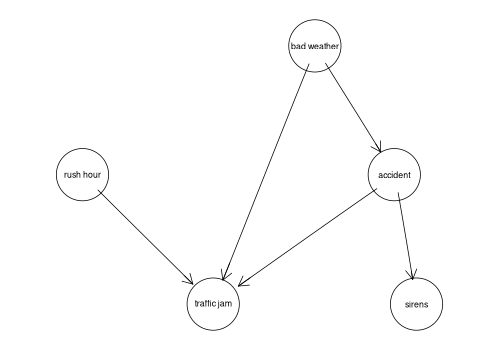
\includegraphics[width=0.75\textwidth]{images/trafficjam.png}
  \caption{A simple example of a DAG \parencite{traffic_jam}}
  \label{dag1}
\end{figure}

Formally, a DAG $G$ is a pair $(V,E)$ where $V$ is a set of \textit{nodes}, one for each of $k$ observable variables, and $E$ is a $V \times V$ set of \textit{edges} or \textit{arcs} \parencite{kalisch2007estimating}. The presence of an edge $(x,y)$ indicates the presence of an directed edge from node $x$ to node $y$. As the name suggests, every edge in $E$ is directed such that if $(x,y) \in E$ then $(y,x) \not \in E$. $E$ is also assumed to not contain any cycles, that is, there is no set of edges ${(i,j)} \in E$ containing a directed path starting and ending at the same node. Figure \ref{dag1} gives a simple example of a DAG.

In general, DAGs can represent either discrete, continuous, or mixed variables, but in the current application only continuous variables will be considered. For simplicity, each arc will hereafter be assumed to define a linear relationship between continuous variables. With this assumption we can more specifically define $V$ as a $(k \times 1)$ vector and $E$ as a $k \times k$ adjacency matrix containing slope parameters, where $e_{ij} \not = 0$ indicates a directed edge from node $i$ to node $j$ and $e_{ij} = 0$ indicates the lack of an edge. The directedness assumption is analogous, and the acyclic property is equivalent to the statement that $E^n$ has zeros on its diagonal for $\forall n > 0$. The model will now also include a $kx1$ vector $\mathbf{\epsilon}$ containing mutually independent Gaussian shocks, one for each node.

The set of nodes from which an arc into $x$ originates are known as the \textit{parents} of $x$ ($pa(x)$), and the set of nodes that have an incoming arc from $x$ are known as the \textit{children} of $x$ ($ch(x)$). The set of all nodes from which a directed path into $x$ originates are known as the \textit{ancestors} of $x$ ($ans(x)$) and the set of all nodes that have an incoming path from $x$ are known as the \textit{decendents} of $x$ ($des(x)$). 

I will now briefly review some key results pertaining to DAGs that are utilised in this paper. For a more complete treatment see \citeauthor{pearl2009causality} (\citeyear{pearl2009causality}).

\theoremstyle{definition}
\begin{definition}{Faithfulness}
  Let $f$ represent some DGP, and $I(f)$ be the conditional independence relationships implied by $f$. A DAG $G$ with parameters $\theta \in \Theta$ is said to be \textbf{faithful} to $f$ if and only if the conditional independence relationships implied by $G$ satisfy $I(G(\theta)) = I(G(\theta^\prime)) = I(f) \text{  } \forall \text{  } \theta \not = \theta^\prime \in \Theta$.
  \parencite[p.48]{pearl2009causality}
  \label{faithfulness}
\end{definition}

Outside of the optional assumption of linearity and Gaussian errors that are made here for simplicity, \textit{faithfulness} is the only assumption necessary for the identification of a DAG for a true DGP. It is the assumption that the conditional independence relationships in the DGP are \textit{stable} to perturbations of parameters. Intuitively, if we wish to use conditional independence relationships to identify a model then we must assume the observed conditional independence relationships do not belie the underlying distribution. This assumption is only violated if some causal effects exactly cancel out, resulting in no observed correlation between casually connected variables. \citeauthor{pearl2009causality} (\citeyear{pearl2009causality}) provides the following example. Consider the following model: $z = \beta_{zx} x + \epsilon_x$, $ y = \beta_{yx} x + \beta_{yz} z + \epsilon_y$. If we impose the parameter restriction $\beta_{yx} = -\beta_{yz}\beta_{zx}$ then $x$ and $y$ are independent. However, this independence relationship is not robust to perturbations of the model parameters and is therefore not stable in the relevant sense. 

A sufficient condition for faithfulness is that the DGP parameters are jointly continuous over the parameter space \parencite{steel2006homogeneity}, or equivalently, that the matrix of DGP parameters is of full rank. This is because under this condition, specific combinations of parameters which result in the cancellation of causal effects have has Lebesgue measure 0. If we believe that the true DGP of the macroeconomy is DSGE model, which itself is faithfully represented by a DAG, then this condition is unlikely to be met. DSGE models impose many cross-equation restrictions on parameters that effectively reduce the rank of the parameter matrix. Unfortunately this condition will not allow us to guarantee that DSGE models satisfy the faithfulness assumption. However, if when considering real macroeconomic data we put aside the assumption that the true DGP is a DSGE model, it does not seem \textit{a priori} unreasonable that the parameter relating, for example, capital and output, and the parameter relating consumption and technology vary independently in different populations. Regardless, this condition is merely sufficient, not necessary, and so it does not rule out that DSGE models can be faithfully represented by DAGs. 

Given this interpretation of faithfulness many readers familiar with the timeseries econometrics literature may recognise a similarity to weak exogeneity \parencite{engle1983exogeneity}. These are indeed closely related concepts, however, they do not entirely overlap. In the context and language of DAGs the definition of a \textit{sequential cut} (necessary for weak exogeneity) given by \citeauthor{engle1983exogeneity} (\citeyear{engle1983exogeneity}) can be interpreted as the statement that the distribution of variables $\mathbf{x}_{t-1}$, $y_t$ and $z_t$ admit factorisation according to the parental markov condition in a DAG where $z_t$ is a parent of $y_t$, and $\mathbf{x}_{t-1}$ is a parent of both and that DAG is faithful (because the parameters are \textit{variation free}). However, unlike weak exogeneity which is defined relative to a parameter, faithfulness is defined relative to a set of conditional independence relationships.

% TODO: Draw small DAG to represent sequential cuts.

In another approach to failures of faithfulness, \citeauthor{steel2006homogeneity} (\citeyear{steel2006homogeneity}) notes that such failures or near-failures (that is near-zero statistical dependence despite clear causal pathways) are likely occur when parameters are both subject to \textit{selection} and \textit{homogeneity}. In this context, selection means that parameters are entirely determined by an economic agent. The suggestion is that if the path of a policy variable $z$ is specifically designed as a function of $x$ to counteract the causal effect of $x$ on some outcome $y$, then it is reasonable to believe that little or no correlation will be observed between $x$ and $y$ despite a clear causal pathway between them. If parameters are assumed to be come from some distribution with different draws for each population, then homogeneity is the statement that there is little exogenous variation in those parameter values, that is variation outside of the variation caused by selection. If \textit{both} selection and homogeneity occur, failure or near-failure of faithfulness is likely to occur. Within the context of macroeconomics, this seems likely to be the case when considering interest rates and the actions of central banks. Assuming the interest rate is set according to a Taylor (\citeyear{taylor1993discretion}) rule, the parameters of that rule are chosen with the specific intent and cancelling the causal effect of inflationary shocks on output and minimizing exogenous variation. 

Despite these concerns, I would argue that the faithfulness assumption is plausible in most macro-economic contexts. For simulations, whether or not the assumption is violated can be read straight off the structural model. For real data, it seems unlikely that any macroeconomic variable (even the policy rate) is determined in an entirely systematic for deterministic way. Identification of policy rate shocks has been a topic of much scrutiny \parencite{ramey2016handbook}, and this line of research has provided a significant amount of evidence for the existence of such shocks. Given that $f$ is \textit{stable} we can use conditional independence tests in the following way to evaluate whether a DAG $G$ is consistent with $f$.

\begin{definition}{D-Separation}
  A path $P$ in a DAG $G$ is said to be \textbf{d-separated} or \textbf{blocked} by a set of variables $\mathbf{z}$ if and only if: \\
  A. $P$ contains a chain $x \rightarrow m \rightarrow y$ or fork $x \leftarrow m \rightarrow y$ and $m \in \mathbf{z}$ \\
  B. $P$ contains a collider $x \rightarrow m \leftarrow y$ and $\{m \cup des(m)\} \cap \mathbf{z} = \emptyset$ \\
  A set of variables $\mathbf{z}$ is said to \textit{d-separate} $x$ and $y$ if $\mathbf{z}$ blocks every path between $x$ and $y$.
  \parencite[p.16]{pearl2009causality}
  \label{dseparation}
\end{definition}

\theoremstyle{theorem}
\begin{theorem}{D-Separation and Conditional Independence}
  If $x$ and $y$ are d-separated by $\mathbf{z}$ in DAG $G$, and $G$ is faithful to the true DGP $f$ of $x$ and $y$, then $x$ and $y$ are independent conditional on $\mathbf{z}$. 
  \parencite[p.16]{pearl2009causality}
\end{theorem}

This result is essential for defining the constraint based tests in section \ref{constrainttests}. In particular, it implies the following result that we will leverage:

\theoremstyle{corollary}
\begin{definition}{Parental Markov Condition}
  Given some DAG $G$, a node $x$ in $G$ is d-separated from and therefore independent of all its non-decendents by its parents. This is known as the \textbf{Parental Markov Condition}. 
  \parencite[p.16, p.19]{pearl2009causality}
  \label{markovcompatibility}
\end{definition}

\theoremstyle{corollary}
\begin{corollary}
  If $G$ is faithful to the DGP $f$ then $f$ admits the following factorisation:
  \begin{equation}
    f(\mathbf{w};\theta) = \prod_{i=1}^{k} f(w_i | pa(w_i);\theta)
  \end{equation}
\end{corollary}

\subsubsection{Estimation} \label{dag_estimation}

There are two fundamental problems to solve when estimating a DAG. The first is known as "parameter learning," and the other "structure learning." Given a DAG as in Figure \ref{dag2}, the first task is simply to estimate the parameters of the network, such as the parameter matrices $\mathbf{A}$, $\mathbf{B}$, $\mathbf{C}$, $\mathbf{D}$, and $\mathbf{E}$ in Equation \ref{ss_solution:x} - \ref{ss_solution:z}. This is usually done via maximum likelihood.

\begin{figure}
  \centering
  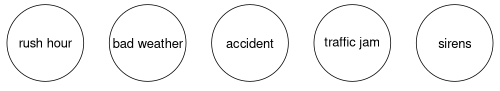
\includegraphics[width=0.75\textwidth]{images/trafficjam_unfit.png}
  \caption{A DAG before structure learning}
  \label{dag2}
\end{figure}

The second task, as demonstrated by Figure \ref{dag2} is that if we just start with some data it is not obvious which conditional probabilities to estimate in the first place. One way to do this is for the researcher to specify explicitly which conditional probabilities should be present in the graph, and simply fit the parameters of that graph. How this can be done in the context of DSGE models is discussed in Section \ref{dsge}. In this context however, doing so achieves little. This is equivalent to specifying a system of linear regressions to be estimated, probably based on some economic model that was developed by other means, and while this is then automatically encapsulated in a convenient, easily interpreted representation of the underlying assumptions, it seems nothing particularly novel would have been achieved. 

A more more exciting approach is to algorithmically learn the structure of the graph, that is to learn a structural model, directly from observed data. One "brute force" method to solving this problem is to compute the posterior likelihood of every possible network, however, this number is super-exponential in the number of variables such that it becomes very computationally expensive, very quickly \parencite{chickering1996learning}. As a response to this, many heuristic approximation techniques have been developed. These can be grouped into two categories: constraint-based and score-based structure learning algorithms \parencite{spirtes1991algorithm} \parencite{verma1991equivalence}. 

\begin{figure}
  \centering
  \begin{subfigure}{0.3\textwidth}
    \centering
    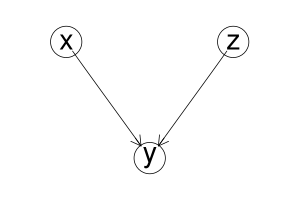
\includegraphics[width=\linewidth]{images/collider.png} 
    \small
    \begin{equation*}
      x = \epsilon_{x}
    \end{equation*}
    \begin{equation*}
      y = \beta_{yx} x + \beta_{yz} z + \epsilon_{y}
    \end{equation*}
    \begin{equation*}
      z = \epsilon_{z}
    \end{equation*}
    \caption{Collider}
    \label{collider}
  \end{subfigure}
  %
  \begin{subfigure}{0.3\textwidth}
    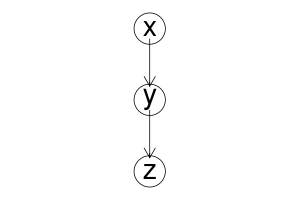
\includegraphics[width=\linewidth]{images/chain.png}
    \small
    \begin{equation*}
      x = \epsilon_{x}
    \end{equation*}
    \begin{equation*}
      y = \beta_{yx} x + \epsilon_{y}
    \end{equation*}
    \begin{equation*}
      z = \beta_{zy} y + \epsilon_{z}
    \end{equation*}
    \caption{Chain}
    \label{chain}
  \end{subfigure}
  %
  \begin{subfigure}{0.3\textwidth}
    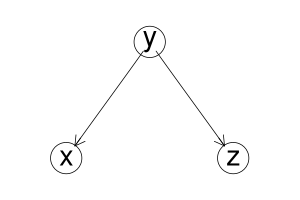
\includegraphics[width=\linewidth]{images/fork.png}
    \small
    \begin{equation*}
      x = \alpha_x + \beta_{xy} y + \epsilon_{x}
    \end{equation*}
    \begin{equation*}
      y = \epsilon_{y}
    \end{equation*}
    \begin{equation*}
      z = \beta_{zy} y + \epsilon_{z}
    \end{equation*}
    \caption{Fork}
    \label{fork}
  \end{subfigure}

  \caption{The three possible v-structures of a 3 node DAG. Error terms $\epsilon$ are all i.i.d. Gaussian shocks.}
  \label{dag5}
\end{figure}

Constraint-based algorithms rely on the fact that changing the direction of an arc changes the conditional independences implied by the graph, the presence of which can be tested for in the data. To see how the DAG assumptions can be sufficient to learn a causal model in this way, consider the example in figure \ref{dag5}. Suppose we have a graph with three nodes, such that no one node is completely independent from the other two (as this would make the graph trivial, and we could in any case rule out this case with an independence test). Furthermore, the graph cannot have all three possible arcs because it would either contain a cycle, or the third arc would imply a relationship which is redundant given the other two. Then the graph must have exactly two arcs. Given this, there are exactly three possible permutations of the network, which are the three shown in figure \ref{dag5}. These are known as the the three canonical "v-structures." \parencite{pearl2014probabilistic} These structures are partially identifiable from observational data because they imply different testable hypotheses about conditional independence. While the chain and fork imply that x and z are unconditionally dependent and only independent conditional on y, the collider implies exactly the opposite; that x and z are unconditionally independent and dependent conditional on y. Given some observed data we can easily test for the presence of conditional and unconditional independence under the assumption of joint-normality using a t-test on (partial) correlations. The results of these tests can be used to rule out certain network structures which would be inconsistent with the observed data. Although for every set of three variables the network is only partially identifiable, full identification can (but will not always) be achieved when more variables are observed, by comparing overlapping triplets of variables and progressively reducing the set of network structures that are consistent both with the DAG assumptions and with the observed conditional independences. There are many that have been implemented using this general approach, the most popular of which is the PC algorithm first developed by \citeauthor{spirtes2000causation} (\citeyear{spirtes2000causation}). This algorithm has been shown to consistently estimate (as $n \rightarrow \infty$) the structure of the ground truth DAG of observed data under the assumptions of linear-Gaussian conditional probability functions, stability, and structural complexity that does not grow too quickly relative to n \parencite{kalisch2007estimating}. 

Score-based methods as the name implies assign some score to every network based on its predictive accuracy and then use gradient-decent to identify the optimum network structure. There are a number of scoring functions and hill climbing algorithms that can be used to achieve this. A consistency result for the GES score-based algorithm is given in \citeauthor{chickering2002optimal} (\citeyear{chickering2002optimal}). The assumptions are slightly stronger than than that of the PC algorithm --- the number of variables must be fixed rather than growing slowly relative to n.

The major benefit of the constraint based method is that it directly utilises conditional independence as a primitive, which is the concept of causality that DAGs seek to identify. This is in contrast to score base methods, which effectively maximise the predictive accuracy of the model, and there is seemingly no guarantee that the most predictive model is the most likely causal explanation. In other words, despite the presence of large sample consistency results for both types of algorithms, it seems likely that small sample bias is more likely to be a problem for score-based methods. The major benefit of score based methods on the other hand is that they will always converge to a single fully directed graph as a solution whereas constraint based methods, because V-structures are only partially identifiable, may not be able to identify a unique solution. Instead, when the graph is only partially identifiable, the algorithm will return an undirected graph (CPDAG). The undirected arcs in a CPDAG could face either direction and the graph would still be consistent with both the DAG assumptions and the observed conditional independences. By permuting the two possible directions of each undirected arc we arrive at a set of graphs that are said to be "observationally equivalent." This is problematic because it is difficult or impossible to fit parameters to graphs that are not fully directed.  

Fortunately, these two methods can be combined into so called "hybrid" structure learning methods which use the strengths of both methods to counter the weaknesses of the other \parencite{scutari2014multiple} \parencite{friedman2013learning}. In this method the algorithm maximises a score function, but the number of parents that each node can have is restricted. The main benefit of this is a large gain computation efficiency because the search space is dramatically reduced, and theoretically it has the benefits of both constraint based and score based learning. However, while resulting the graph is always directed, it does not always correctly reflect the observed v-structures because it trades off constraint satisfaction and score maximisation. \citeauthor{nandy2018high} (\citeyear{nandy2018high}) gives an asymptotic consistency result for the ARGES hybrid learning algorithm.

\subsection{DSGE Models} \label{dsge}

Suppose a DSGE model is defined over a set of $k$ variables in a vector $\mathbf{w}$. The solution to a log-linearised DSGE model can be written as a state space model \parencite{king1988production} that partitions $\mathbf{w}$ into three mutually exclusive vectors $\mathbf{x}$, $\mathbf{y}$, and $\mathbf{z}$. This state-space model is described by equations \ref{ss_solution:x} - \ref{ss_solution:z}:

\begin{align}
  \mathbf{y}_t &= \mathbf{A} \mathbf{x}_{t-1} + \mathbf{B} \mathbf{z}_{t} \label{ss_solution:x}\\
  \mathbf{x}_t &= \mathbf{C} \mathbf{x}_{t-1} + \mathbf{D} \mathbf{z}_{t} \label{ss_solution:y}\\
  \mathbf{z}_t &= \mathbf{E} \mathbf{z}_{t-1} + \mathbf{\epsilon}_{t} \label{ss_solution:z}
\end{align}

Where $\mathbf{x}_t$ is a vector of control variables, $\mathbf{y}_t$ is a vector of endogenous state variables, $\mathbf{z}_t$ is a vector of exogenous state variables, $\mathbf{A}$, $\mathbf{B}$, $\mathbf{C}$ and, $\mathbf{D}$ are coefficient matrices, and $\mathbf{\epsilon}_t$ is a vector of shocks. All variables are mean-zero. The shocks in $\mathbf{\epsilon}_t$ can be interpreted as structural shocks as they satisfy the assumptions $\mathbf{\epsilon}_{t} \sim N(0,\Sigma)$ and $\Sigma$ diagonal $\implies Cov[\epsilon_{i,t},\epsilon_{j,t}] = 0 \iff \epsilon_{i,t} \indep \epsilon_{j,t} $ for $i \not = j$. These shocks are assumed to not be observed, both because this is likely true in realistic applications (absent some very clever econometric tricks) and because observing the shocks is not necessary for the inference proposed here.

Furthermore assume that $\mathbf{E}$ is diagonal ($e_{ij} = 0$ if $i \not = j$) such that the process of each exogenous state depends only on its own past and $|e_{ii}| < 1$ such that the model has a stationary solution. Note that for simplicity the exogenous states are assumed to possess the Markov property, that is, $\mathbf{z}_t$ depends only on $\mathbf{z}_{t-1}$ and not any further lags. As a result, the entire model has the Markov property. However, the framework and algorithm proposed here could easily be generalised to allow for longer lags.

In this setup, all variables can be categorized as either state variables or control variables \parencite{fernandez2016solution}. Defined as broadly as possible, state variables are the variables whose past is relevant for determining the current value of modelled variables, and control variables are the rest; their past is independent of the current values of the model. State variables can be further categorized as either endogenous states (such as the capital stock) and exogenous states (such as the state of technology or productivity) \parencite{ravenna2007vector}. As the name suggests, endogenous states are determined simultaneously (endogenously) with contemporaneous controls in the model, however, their past is by definition exogenous and relevant to the determination of the current values of the model. Exogenous states, on the other hand, are exogenous in the sense that they are determined independently of any contemporaneous variables in the model, and are thus determined entirely by the past of the model or any exogenous innovations (shocks) that might be present. The distinction between endogenous and exogenous states is subtle, and it is primarily made because we often wish to give different interpretations to these two types of variables, but the fact that exogenous states enter the prediction of time $t$ endogenous variables at time $t$ rather than at time $t-1$ is an important modelling distinction.

\section{Methodology}

Given equations \ref{ss_solution:x} - \ref{ss_solution:z} it is straightforward to characterize the general solution to a DSGE model as a DAG. This is demonstrated by Figure \ref{dsge_dag}. This expresses in graphical format all of the assumptions outlined in those equations. 

\begin{figure}
  \centering
  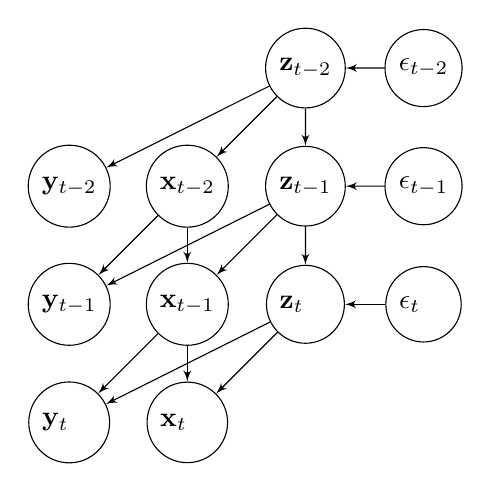
\begin{tikzpicture}[scale=1.5]
    \tikzset{
      vertex/.style={circle,draw, minimum size=2em},
      edge/.style={->,> = latex'}
    }
    % vertices
    \node[vertex] (zt) at (1 ,0) {$\mathbf{z}_{t\quad}$};
    \node[vertex] (zt1) at (1 , 1) {$\mathbf{z}_{t-1}$};
    \node[vertex] (zt2) at (1 , 2) {$\mathbf{z}_{t-2}$};
    \node[vertex] (xt) at (0 ,-1) {$\mathbf{x}_{t\quad}$};
    \node[vertex] (xt1) at (0 , 0) {$\mathbf{x}_{t-1}$};
    \node[vertex] (xt2) at (0 , 1) {$\mathbf{x}_{t-2}$};
    \node[vertex] (yt) at (-1,-1) {$\mathbf{y}_{t\quad}$};
    \node[vertex] (yt1) at (-1, 0) {$\mathbf{y}_{t-1}$};
    \node[vertex] (yt2) at (-1, 1) {$\mathbf{y}_{t-2}$};
    \node[vertex] (et) at (2 , 0) {$\mathbf{\epsilon}_{t\quad}$};
    \node[vertex] (et1) at (2 , 1) {$\mathbf{\epsilon}_{t-1}$};
    \node[vertex] (et2) at (2 , 2) {$\mathbf{\epsilon}_{t-2}$};

    %edges
    \draw[edge] (et) -- (zt);
    \draw[edge] (et1) -- (zt1);
    \draw[edge] (et2) -- (zt2);
    \draw[edge] (zt2) -- (zt1);
    \draw[edge] (zt1) -- (zt);
    \draw[edge] (xt2) -- (xt1);
    \draw[edge] (xt1) -- (xt);
    \draw[edge] (zt2) -- (xt2);
    \draw[edge] (zt1) -- (xt1);
    \draw[edge] (zt) -- (xt);
    \draw[edge] (zt2) -- (yt2);
    \draw[edge] (zt1) -- (yt1);
    \draw[edge] (zt) -- (yt);
    \draw[edge] (xt2) -- (yt1);
    \draw[edge] (xt1) -- (yt);
  \end{tikzpicture}
  \caption{DSGE solution expressed as a DAG}
  \label{dsge_dag}
\end{figure}

Given this it would seem straightforward to input random samples generated from a DSGE model into the available structure learning algorithms and find the correct solution, given that these algorithms have well established asymptotic convergence properties. Unfortunately, despite extensive experimentation with these tools, I was unable to obtain any results in this way, as these algorithms seem to have a number of important limitations in this context. Constraint-based algorithms rely on conditional independence tests which themselves involve computing the correlation between residuals. In the context of simulated data these residuals may be very small or effectively zero when conditioning on the true parents of a node. In this case the computation of partial correlations may be unstable and lead to spurious results. Furthermore, these results are only asymptotic and it seems that finite-sample bias may be important in economic applications, where sample sizes are small. Particularly problematic is that structure learning algorithms consider all possible DAGs given observed variables as potential candidates, whereas in this context we assume that the solution takes on a particular form, as in \ref{dsge_dag}.

As a result of these limitations, a more effective approach in this context is to design a bespoke algorithm that takes into account the relatively stringent assumptions that can be made about DSGE solutions. For the reasons outlined in section \ref{dag_estimation} this will be a hybrid algorithm. Therefore, before introducing the algorithm we will define relevant constraint and score tests in turn.

\subsection{Constraint Tests} \label{constrainttests}

Figure \ref{dsge_dag} implies the following four independence relationships among the time $t$ and $t-1$ variables:

\begin{align}
  x_t \indep y_t \,||\,& [\mathbf{x}_{t-1},\mathbf{z}_t] \text{ for all } (x_t, y_t) \in [\mathbf{x}_t, \mathbf{y}_t] \label{constraint_test:1} \\
  x_{t-1} \indep z_{t} \,||\,& \mathbf{z}_{t-1} \text{ for all } x_{t-1} \in \mathbf{x}_{t-1} \text{ and } z_{t} \in \mathbf{z}_t \label{constraint_test:3} \\
  x_t \indep z_{t-1} \,||\,& [\mathbf{x}_{t-1}, \mathbf{z}_t] \text{ for all } x_t \in [\mathbf{x}_t, \mathbf{y}_t] \text{ and } z_{t-1} \in \mathbf{z}_{t-1} \label{constraint_test:2} \\
  z_t \indep z^{\prime}_{t} || \mathbf{z}_{t-1} & \text{ for all } z_t \not = z^{\prime}_{t} \in \mathbf{z}_t \label{constraint_test:4}
\end{align}

The first condition (\ref{constraint_test:1}) is the statement that the model's time $t$ endogenous variables are explained entirely by and are therefore unconfounded conditional on $\mathbf{x}_{t-1}$ and $\mathbf{z}_t$ (the time $t$ states). In DAG parlance, a time $t$ endogenous variable is \textit{d-separated} from and therefore independent of any other time $t$ endogenous variable by the time $t$ states. Condition (\ref{constraint_test:3}) states that the time $t$ states that every lagged endogenous state is independent of every exogenous state conditional on the lagged exogenous states. This follows from the exogeneity of $\mathbf{z}$ which implies that the only parent of $z_t$ other than the shock is $z_{t-1}$. Condition (\ref{constraint_test:2}) holds because the time $t$ states d-separate the time $t$ endogenous variables from the lagged exogenous states. If we were to consider further lags, this conditional independence would apply not only to $z_{t-1}$, but also to all $t-2$ and earlier variables because of the Markov condition. Finally, Condition (\ref{constraint_test:4}) holds that all exogenous states are mutually independent conditional on past exogenous shocks. This is a stronger assumption than the other three, and depends crucially on the assumption that the shocks $\mathbf{\epsilon}_t$ are mutually uncorrelated, and thus structural in nature.

These constraint tests already provide a powerful selection criteria for empirical DSGE models I will call DAG-validity:

\begin{definition}
  For a set of variables $\mathbf{w}$ a log-linearised DSGE model $M$ is \textit{valid} with respect to a distribution $f(\mathbf{w})$ if the exogenous states ($\mathbf{z}$), endogenous states ($\mathbf{x}$) and controls ($\mathbf{y}$) of $M$ as defined in equations (\ref{ss_solution:x}) - (\ref{ss_solution:z}) satisfy conditions (\ref{constraint_test:1}) and (\ref{constraint_test:3}).
  \label{validity}
\end{definition}

It is proved in an appendix (\ref{proofs}) that validity is necessary and sufficient to guarantee that if the ground truth can be characterised as in (\ref{ss_solution:x}) - (\ref{ss_solution:z}) then DSGE models that are dag-consistent with the ground truth have the same DAG representation, and therefore, the same state-space model. Constraints (\ref{constraint_test:2}) and (\ref{constraint_test:4}) are still applicable because they are implied by the DAG, but there are not required. To be more general we could drop these assumptions as long as the shocks only directly effect the exogenous states, and the other constraints would still hold and be valid tests of the model. However, these constraints (and the associated assumptions) are nonetheless included because they is satisfied by a wide range of DSGE models including all of those considered in the empirical portion of this paper, and all else equal conducting a larger number of tests gives more statistical \textit{power} to reject incorrect models when using finite samples.

\subsection{Score Tests} \label{scoretests}

The most basic score function for Gaussian Bayesian networks is the log-likelihood function. The Markov compatibility condition (Definition \ref{markovcompatibility}) DAG admits factorisation of the joint probability distribution into the product of the distribution of each variable conditional on its parents:

\begin{equation}
  f(\mathbf{w};\theta) = \prod_{i=1}^{k} f(w_i | pa_i;\theta)
\end{equation}

Therefore, the log-likelihood can be calculated as:

\begin{equation}
  \mathcal{L}(\mathbf{w},\theta) = \sum_{i=1}^{k} ln(f(w_i | pa_i;\theta))
\end{equation}

Now consider the assumptions in the current context. $\mathbf{w_i}$ is partitioned into $\mathbf{z}$, $\mathbf{x}$, and, $\mathbf{y}$. We assume that the conditional probabilities are linear functions and follow a mean-zero normal distribution, so the only parameter is the variance-covariance matrix $\mathbf{sigma}^2$. Furthermore, values from period $t-1$ are known at time $t$ and therefore these root nodes are deterministic, so their distribution is trivial. Therefore,

\begin{align}
  \mathcal{L}(\mathbf{w}; \mathbf{A}, \mathbf{B}, \mathbf{C}, \mathbf{D}, \mathbf{E}, \mathbf{\sigma}^2) =& \sum_{z_{i,t} \in \mathbf{z}_t} \bigg{(} \sum_{t=1}^{T} ln(\phi(z_{i,t} | z_{i,t-1} | \mathbf{E}, \mathbf{\sigma}^2)) \bigg{)} \nonumber\\
  +& \sum_{y_{i,t} \in [\mathbf{y}_t,\mathbf{x}_t]} \bigg{(} \sum_{t=1}^{T} ln(\phi(y_{i,t} | [\mathbf{x}_{t-1}, \mathbf{z}_{t}] | \mathbf{A}, \mathbf{B}, \mathbf{C}, \mathbf{D}, \mathbf{\sigma}^2)) \bigg{)} \\
  =& \sum_{y_{i,t} \in \mathbf{y}_t} \bigg{(} \sum_{t=1}^{T} ln(\phi(\mathbf{a}_i \mathbf{x}_{t-1} + \mathbf{b}_i \mathbf{z}_t | \mathbf{a}_i, \mathbf{b}_i, \sigma_{y_i}^2)) \bigg{)} + \nonumber\\
  & \sum_{x_{i,t} \in \mathbf{x}_t} \bigg{(} \sum_{t=1}^{T} ln(\phi(\mathbf{c}_i \mathbf{x}_{t-1} + \mathbf{d}_i \mathbf{z}_t | \mathbf{c}_i, \mathbf{d}_i, \sigma_{x_i}^2)) \bigg{)} \nonumber\\
  & \sum_{z_{i,t} \in \mathbf{z}_t} \bigg{(} \sum_{t=1}^{T} ln(\phi(\mathbf{e}_i z_{i,t-1}  | \mathbf{e}_i, \sigma_{z_i}^2)) \bigg{)}
\end{align}

Where $\mathbf{x_i}$ is the $i_{th}$ row of $\mathbf{X_i}$. Notice that we can calculate the variances separately in each regression because the Markov compatibility condition implies that they are independent. Finally, we can substitute in for the maximum likelihood estimate of $\sigma^2$ for each regression and the functional form of $\phi$ to arrive at an expression for the log-likelihood function:

\begin{align}
  \mathcal{L(\mathbf{w})} =& -\frac{T}{2} \bigg{(} 
  k (1 + ln(2\pi)) 
  + \sum_{i=1}^{k} ln(\hat{\sigma}_{i}^2)
  \bigg{)} \\
  \hat{\sigma}_{i}^2 =& \frac{1}{T} \sum_{t=1}^{T} (w_{i,t} - \hat{w}_{i,t})^2
\end{align}

Where $\hat{w}_{i,t}$ is are of predicted values of some $w_i$ in $\mathbf{w}$ implied by estimates of equations (\ref{ss_solution:x}) - (\ref{ss_solution:z}) using the maximum-likelihood estimates of the coefficient matrices.

Since maximising the log-likelihood does not penalise complexity, it often favours models with many more edges than exist in the ground truth. In other words, maximising log-likelihood over a space of candidate DAGs may lead to \textit{overfitting}. As a result there are many penalised score functions based on the log-likelihood that are available. Here we consider two of the most popular, the Akaike Information Criterion (AIC) \parencite{akaike1974new} and the Bayesian Information Criterion (BIC) \parencite{schwarz1978estimating}, which are calculated as follows:

\begin{align}
  AIC(\mathbf{w}) =& 2k - 2\mathcal{L}(\mathbf{w})\\
  BIC(\mathbf{w}) =& kln(T) - 2\mathcal{L}(\mathbf{w})
\end{align}

Where $k = 2[|\mathbf{z}| + (|\mathbf{z}| + |\mathbf{x}|)(|\mathbf{y}| + |\mathbf{x}|)]$ is the total number of estimated parameters. Given that the algorithm terminates when a minimal valid set of states has been found, it may seem that this bias towards complexity is irrelevant. However given the minimal number of states, it is still possible to reallocate between exogenous and endogenous states. In this context the bias towards complexity means a we are likely to choose more exogenous states than truly exist, since these involve the estimation of more parameters than endogenous states, and since they enter at time $t$ instead of time $t-1$ they likely contain more relevant information about time $t$ endogenous variables. Therefore, it is still beneficial to score valid models in a penalised way.

\subsection{Algorithm} \label{algo}

\begin{minipage}{\linewidth}
  \begin{algorithm}[H]
    \SetAlgoLined
    \DontPrintSemicolon
    
    % python like syntax
    \SetStartEndCondition{ }{}{}%
    \SetKwProg{Fn}{def}{\string:}{}
    \SetKwFunction{Range}{range}%%
    \SetKw{KwTo}{in}\SetKwFor{For}{for}{\string:}{}%
    \SetKwIF{If}{ElseIf}{Else}{if}{:}{elif}{else:}{}%
    \SetKwFor{While}{while}{:}{fintq}%
    \AlgoDontDisplayBlockMarkers
    \SetAlgoNoEnd
    %\SetAlgoNoLine

    \SetKwData{Continue}{$continue$}
    \SetKwData{Nstates}{$n\_states$}
    \SetKwData{Maxstates}{$max\_states$}
    \SetKwData{Allvalidstates}{$all\_valid\_states$}
    \SetKwData{Siglevel}{$sig\_level$}
    \SetKwData{Potentialstates}{$potential\_states$}
    \SetKwData{Allpotentialstates}{$all\_potential\_states$}
    \SetKwData{Potentialstate}{$potential\_state$}
    \SetKwData{Constrainttests}{$constraint\_tests$}
    \SetKwData{Constrainttest}{$constraint\_test$}
    \SetKwData{Scoretests}{$score\_tests$}
    \SetKwData{Scoretest}{$score\_test$}
    \SetKwData{States}{$states$}
    \SetKwData{True}{$true$}
    \SetKwData{False}{$false$}
    \SetKwFunction{Getpotentialstates}{$get\_potential\_states$}
    \SetKwData{Getconstrainttests}{$get\_constraint\_tests$}
    \SetKwData{Getscoretests}{$get\_score\_tests$}
    \KwIn{$alpha$: significance level}
    \KwOut{$all\_valid\_states$: A set of minimal sets of exogenous and endogenous states whose implied conditional independences are valid relative to the observed data}
    \Begin{
      \Continue $=$ \True\;
      \Nstates $= 0$\;
      \Maxstates $= \#observables - 1$\;
      \Allvalidstates $= list()$ \;
      \While{\Continue $and$ \Nstates $<=$ \Maxstates} {
        \Allpotentialstates $=$ \Getpotentialstates{\Nstates}\;
        \For{\Potentialstates $\in$ \Allpotentialstates}{
          \Constrainttests $=$ \Getconstrainttests{\Potentialstates}\;
          \Scoretests $=$ \Getscoretests{\Potentialstates}\;
          \Siglevel $=$ $\frac{alpha}{length(constraint\_tests)}$\;
          \If{$every$ \Constrainttest $.p\_value >$ \Siglevel $for$ \Constrainttest $\in$ \Constrainttests}{
            $append$ \Potentialstates $to$ \Allvalidstates\;
            \Continue $=$ \False\;
          }
        }
      }
      $sort$ \Allvalidstates $by$ \Scoretests\;
      $return$ \Allvalidstates
  }
    \caption{Brute force hybrid state-space estimation algorithm}
    \label{constraint_algo}
  \end{algorithm}
\end{minipage} \\

The algorithm is very simple and is designed to reflect a few model selection heuristics. 

The algorithm also assumes that the constraints validity is more important than score maximisation. The scores of models that are not valid relative to the constraints are irrelevant because these models are thrown out. The justification for this heuristic is outlined int \ref{dag_estimation}. Essentially, unlike score functions, constraints directly encode information about a relevant sense of causality.

The algorithm applies the Minimal State Variable (MSV) criteria \parencite{mccallum1999role}. Once a model is found that is valid relative to the conditional independence tests, models with more states are not considered because these are inferior solutions. There are a number of relevant justifications for the application of this criteria. Firstly, this can be seen as the application of \textit{Occam's Razor} to state-space models, wherein state variables have more complex dynamics than controls. Consider equations (\ref{ss_solution:x}) - (\ref{ss_solution:z}). Exogenous states are involved in all three equations, endogenous states two, and controls only one. Another way to see this is in figure \ref{dsge_dag}. Among time $t$ and $t-1$ variables, adding an exogenous state results in the addition of edges in four places, an endogenous state in three places, and a control in only two. Therefore, models with with fewer states, especially exogenous states are more parsimonious and are therefore preferable, all else equal. The MSV criteria also allows for a potentially very large increase in the speed of the algorithm. Without it we must consider every possible combinations of states. Since the choice of states is multinomial with three categories the complexity of this algorithm is $\mathcal{O}(3^k)$. However, if the ground truth has only $m < k$ states then we can skip $\sum_{r=m}^{k} 2^r {\binom{k}{r}}$ iterations, which is potentially many orders of magnitude if $m << k$. This algorithm is nonetheless highly inefficient, however, given that macroeconomic data is usually of relatively low dimension, it is still feasible in many important cases. There are undoubtedly many performance improvements which could be made to this algorithm, but this is left as a topic for for future research.

Given the fact that this algorithm considers every possible state-space model, and the result in \ref{constrainttests}, if conditional independence was completely observable this algorithm would always identify the ground truth state-space model. Unfortunately, in empirical applications with finite samples we have to rely on conditional independence tests that are not always correct. Since observed variables are assumed to follow a normal distribution, zero (partial) correlation is the same as (conditional) independence. So the conditional independence test that is used in this application is a t-test on the (partial) correlation of the relevant variables. It is important to note that these conditional independence tests are used in a somewhat unusual manner. Unlike most economic applications, the case we are interested in is the case in which we \textit{do not reject} the null hypotheses that the correlation is 0. In each test, the significance level $\alpha$ is the probability of rejecting the hypothesis that the true (partial) correlation is 0, and therefore, rejecting the model under consideration. 

For any given model we may consider a large number of conditional independence tests (the number is polynomial order in the number in each category), and so there is a multiple comparisons problem. In an attempt to correct for this a Bonferroni (\citeyear{bonferroni1936teoria}) correction is applied. The Bonferroni correction adjusts the significance level assuming the independence of tests. In this context tests are clearly not independent, therefore, given the correction, $\alpha$ should be interpreted as an upper bound on the probability of rejecting a correct model.

When investigating a statistical methodology there are two broad categories of properties that we may wish to establish. First are the asymptotic properties relating to the identifiability of the parameters of interest. In this context the goal is to establish that the algorithm selects the correct ground truth state-space model as the number of observations $n$ goes to infinity. It is straightforward to (at least informally) demonstrate the asymptotic consistency of this algorithm. Consider data generated from a DGP characterised by (\ref{ss_solution:x}) - (\ref{ss_solution:z}) that satisfies (\ref{constraint_test:1}) - (\ref{constraint_test:4}). Sample (partial) correlation is a consistent estimator of (partial) correlation, so the partial correlations estimated for (\ref{constraint_test:1}) - (\ref{constraint_test:4}), and thus the probability of rejecting the true model goes to zero as $n \rightarrow \infty$. On the other hand, consider a DSGE model that does not have the same state-space representation as the DGP. The result in \ref{proofs} implies that at least one of these the partial correlations in (\ref{constraint_test:1}) - (\ref{constraint_test:3}) is not zero, and therefore, the associated sample partial correlation does not converge to zero as $n \rightarrow \infty$. The t-statistic for this partial correlation goes to infinity and the chance of rejecting this incorrect model goes to 1 as $n \rightarrow \infty$.

The other properties to consider are the finite sample or statistical inference properties. These may be much more difficult to establish because the probability that the correct model is not chosen depends both on the probability that some other incorrect model is \textit{valid}, and that that incorrect model has a higher score than the correct model. Both of these probabilities, in turn, depend on the alternative incorrect model under consideration. Therefore, instead of considering any theory in this regard, I will use simulations to demonstrate performance on finite samples in \ref{results}.

\subsection{Related Modelling Techniques}

Having discussed how DSGE models and macroeconomic data more generally can be represented as DAGs this section will discuss how this approach relates to other econometric approaches which are common in the analysis of macroeconomic timeseries. It is possible to draw comparisions with both Structural Vector Autoregression (SVAR) and Autoregessive Distributed Lag (ADL) models, so these will be discussed in turn.

One of the most common and simplest econometric models for this type of data is the vector autoregression (VAR), which was introduced by \citeauthor{sims1980macroeconomics} (\citeyear{sims1980macroeconomics}). This method involves regressing a vector of outcomes $y_t$ on a matrix containing $k$ lags of $y$ in the form $y_t = [y_{t-1}, ..., y_{t-k}] \beta + \epsilon_t $. The primary concern with and limitation of this approach is that the estimated covariance matrix $\epsilon_t$ is unrestricted, so the shocks contained within it are not mutually independent. Therefore, this model can not be used to estimate the effect of a truely exogenous shock on the dynamics of observed variables. In order to address this issue the model is transformed and an assumed causal ordering is imposed in the form of a Cholesky decomposition \parencite{sims1980macroeconomics}, which has the effect of making the errors of the estimated, transformed model mutally uncorrelated or \textit{structural}. Therefore, such models are known as SVARs. As noted by \citeauthor{demiralp2003searching} (\citeyear{demiralp2003searching}), in this context there is an equivallence between SVAR models and DAGs. This is because root nodes are assumed to be mutually uncorrelated, and as a result, any shocks to these will have a structural interpretation.

However, one key difference between a DAG in this context and a SVAR model is that the DAG allows for some variables to depend on contemporanious values of other variables. In particular, the endogenous states and controls depend contemporaniously on the exogenous states. In this sense the DAG is similar to an ADL model. When implementing an ADL model it is necessary for the researcher to choose which contemporanious variables to include as regressors, implicitly assuming that this regressors are at least predetermined relative to the outcomes of interest. 

The primary advantage of DAGs is the relatively weak assumptions they require. Both the SVAR and ADL models require the researcher to specify assumptions about the relative exogeneity of observable variables. These assumptions are themselves either derived from a similarly assumption-heavy model such as a DSGE model, or are entirely \textit{ad hoc}. There has been a long tradition within the field of economics including seminal papers by \citeauthor{lucas1976econometric} (\citeyear{lucas1976econometric}), \citeauthor{sims1980macroeconomics} (\citeyear{sims1980macroeconomics}), and \citeauthor{jorda2005estimation}, (\citeyear{jorda2005estimation}) criticising this type of model building. DAGs, along with structure learning algorithms provide an asymptotically consistent, agnostic, and data-driven alternative to models of this kind.

\subsection{Model Evaluation}

Since the state-space models that are estimated here are fundamentally reduced-form models they will not circumvent the Lucas (\citeyear{lucas1976econometric}) critique. When the state-space model is estimated directly from a micro-founded DSGE model these coefficient matrices are functions of the structural parameters of that model. However, when these matrices are estimated directly from data they can not, and should not be interpreted as structural parameters. The methodology in this paper is one of \textit{model selection}, that is, evaluating whether a given DSGE model is consistent with observational data. 

\subsection{IRFs}

One very common way of evaluating DSGE models is to compare the Impulse Response Functions (IRFs) they imply and to compare those with the IRFs of reduced form models such as VAR models \parencite[p.83]{ramey2016handbook}. This is also possible when directly estimating state-space models, and the results of this will be considered in the empirical section of this paper. IRFs are calculated, starting with a vector of initial values (shocks), by iteratively using the estimated matrices $\hat{\mathbf{A}}$ = $\hat{\mathbf{E}}$ to calculate current time step values using past values. Note that this can be done for either exogenous or endogenous states, but not for controls, as changes to these are by construction not propagated through to future time steps.

\section{Data}

In order to demonstrate the capability of the DAG methodology empirically I will work with both simulated and real macroeconomic data. Using simulated data has a number of key advantages. Firstly, since the model that simulates the data is known it is possible to evaluate whether the structure learning has succeeded in identifying the ground truth DAG. Secondly, in this context it is possible to ensure to the greatest possible extent that the underlying assumptions of the structure learning algorithms, including linearity and normality are satisfied. Finally, since these models are central to modern macroeconomics it provides a controlled testing environment which is also arguably highly relevant to real data. On the other hand, using real data is an opportunity to demonstrate that DAGs are also a powerful heuristic tool that can be implemented outside of a rigorously controlled environment. The remainder of this section will discuss the various sources and general properties of the data used in this paper.

\subsection{Simulations}

In order to collect simulated data I consulted a github repository containing Dynare code to replicate a number of well known macroeconomic models \parencite{pfeifer2020}. In particular, I chose to model the baseline RBC model as a simple case and the \citeauthor{smets2007shocks} (\citeyear{smets2007shocks}) model for a more difficult and complex modelling challenge. I modified the simulation code slightly such that simulations would output a file containing $n$ observations of $i.i.d.$ draws of the exogenous shocks, and the associated observed values of the other variables in the model. This file was then used as the input for fitting DAGs.

\subsubsection{Baseline RBC}

\begin{table}
  \centering
  \begin{tabular}{|l|l|l|}
    \hline
    Symbol & Name & Type \\
    \hline
    $g$ & government spending & exogenous state \\
    $z$ & technology & exogenous state \\
    $k$ & capital & endogenous state \\
    $w$ & wage rate & control \\
    $r$ & return to capital & control \\
    $y$ & output & control \\
    $c$ & consumption & control \\
    $l$ & hours worked & control \\
    $i$ & investment & control \\ \cline{2-2}
    \hline
  \end{tabular}
  \caption{Description of Variables for the baseline RBC model.}
  \label{rbc_data}
\end{table}

The first model which I have chosen to evaluate is the baseline RBC model provided by \citeauthor{pfeifer2020} (\citeyear{pfeifer2020}). This model includes 11 variables which are summarised by table \ref{rbc_data}. This model contains two exogenous state variables: technology ($z$) and government spending ($g$), and one endogenous state: capital ($k$). There are two shocks in the model: $eps_z$ that affects only technology directly and $eps_g$ that affects only government spending directly, but as explained in section \ref{dsge} these are dropped from the data.

This model was chosen as it is one of the simplest DSGE models and provides a good baseline to demonstrate the effectiveness of this methodology. In particular, the default calibration of this model which was used has autoregressive coefficients on the exogenous technology and government spending processes that are very close to one, and as a result there is a high degree of persistence in all variables in the model. this model will test the algorithms performance when the assumption of stationarity is challenged.

\subsubsection{Baseline New Keynsian}

\begin{table}
  \centering
  \begin{tabular}{|l|l|l|}
    \hline
    Symbol & Name & Type \\
    \hline
    $nu$ & policy rate & exogenous state \\
    $a$ & technology & exogenous state \\
    $z$ & preferences & exogenous state \\
    $p$ & price level & endogenous state \\
    $y$ & output & control \\
    $i$ & nominal interest & control \\
    $pi$ & inflation & control \\
    $r\_nat$ & natural interest rate & control \\
    $r\_real$ & real interest rate & control \\
    $n$ & hours worked & control \\
    $m\_real$ & real money balances & control \\
    $w\_real$ & real wages & control \\
    $mu$ & mark-up & control \\ \cline{2-2}
    \hline
  \end{tabular}
  \caption{Description of Variables for the baseline New Keynesian model.}
  \label{nk_data}
\end{table}

New Keynesian models are extremely popular in modern macroeconomics and are thus a worthy test for this methodology. In particular, I use a model from \citeauthor{gali2015monetary} (\citeyear{gali2015monetary}) as provided by \citeauthor{pfeifer2020} (\citeyear{pfeifer2020}). The variables in this model are summarised in table \ref{nk_data}  \footnote{Some control variables which were perfectly correlated with another variable were dropped, for example, annualised rates.}. This model has a total of four states: three exogenous (policy rate, technology and, preferences) for which there is one i.i.d. shock each, and one endogenous (price level).

\subsection{US Data}

\begin{table}
  \centering
  \begin{tabular}{|l|l|}
    \hline
    Symbol & Name \\
    \hline
    $pi$ & CPI Inflation \\
    $rm$ & Federal Funds Rate (Return to Money) \\
    $g$ & (Real) Government Expenditure \\
    $y$ & (Real) GDP \\
    $i$ & (Real) Private Investment \\
    $w$ & Median (Real) Wage \\
    $rk$ & Return to Capital \tablefootnote{Estimated as average return to the NASDAQ over the relevant period} \\
    $z$ & Total Factor Productivity \\
    $u$ & Unemployment \\
    $l$ & Total Workforce \\
    $c$ & (Real) Personal Consumption \\\cline{2-2}
    \hline
  \end{tabular}
  \caption{Description of Variables for US Data}
  \label{tab3}
\end{table}

To provide an example of real macroeconomic time-series, quarterly data from the US between years 1985-2005 were collected from FRED (\citeyear{fred2020data}) for 15 variables outlined in Table \ref{tab3}. All of the variables were detrended by taking the residuals of an estimated first order autoregression. Total factor productivity and capital stock were provided on an annual basis and were therefore interpolated quadratically. Full details of data preprocessing are available in the project repository \parencite{hall2020git}.

\section{Results} \label{results}

In this section many of the properties of the proposed algorithm will be thoroughly investigated. Using simulated data allows for the possibility of many experiments to test these properties in a controlled environment. In particular, for the models under consideration two tests will be considered, one for each of the algorithmic properties outlined in section \ref{algo}. To demonstrate asymptotic consistency, results from the algorithm for a very large number of samples (100,000) will be provided. To demonstrate the finite sample properties, results from a large number of runs of the algorithm (1000) with a relatively small sample size (100, the sample size of the real data) will be provided and discussed.

\subsection{Baseline RBC}

Using a the entire sample for the RBC model the algorithm successfully identifies the correct states, and no other (incorrect) models are valid. Figure \ref{rbc_irfs} shows the impulse responses to a technology shock generated by the original simulation and the estimated model. There are almost identical, as they should be. This is a simple validation of the state-space representation and that fact that we have recovered the correct parameters using observational maximum likelihood.

\begin{figure}
  \centering
  \begin{subfigure}{0.8\textwidth}
    \centering
    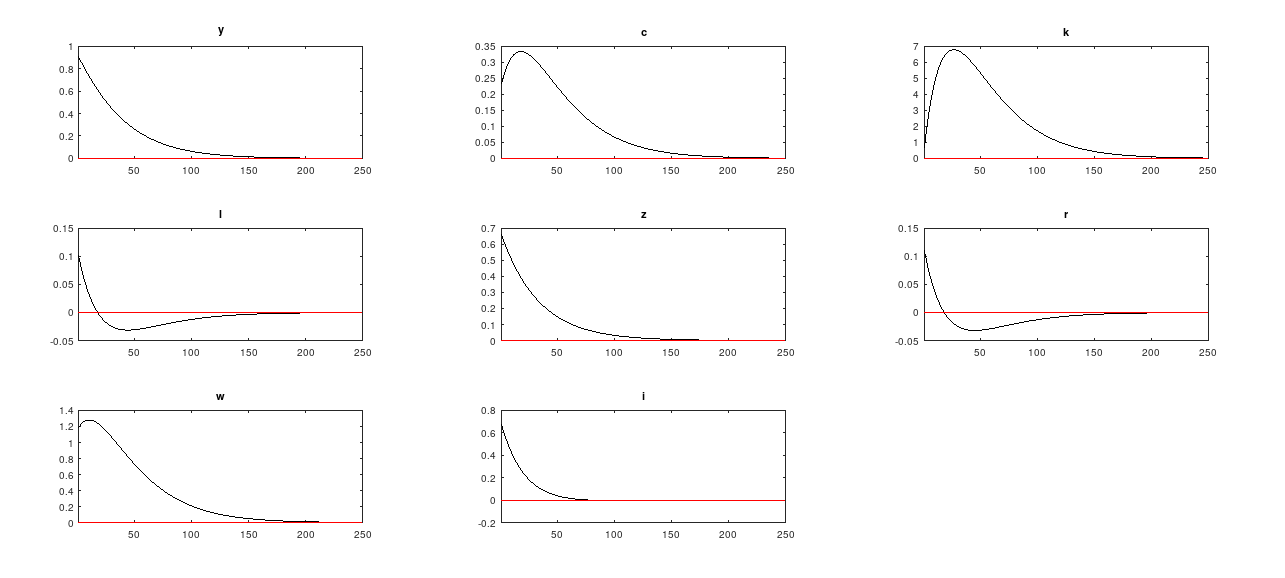
\includegraphics[width=\linewidth]{images/rbc_sim_irf.png} 
    \caption{Original Simulation}
    \label{rbc_simirf}
  \end{subfigure}
  %
  \begin{subfigure}{0.8\textwidth}
    \centering  
    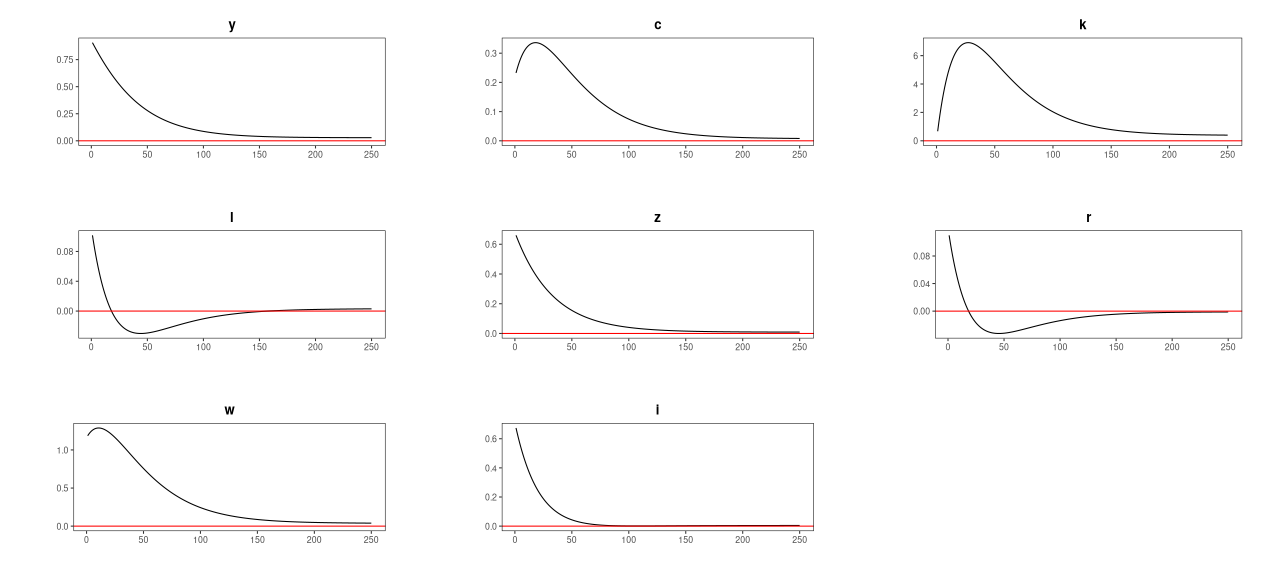
\includegraphics[width=\linewidth]{images/rbc_true_dag_irfs.png}
    \caption{Ground Truth DAG / Estimated DAG}
    \label{rbc_gtirf}
  \end{subfigure}

  \caption{IRFs to a one standard deviation technology shock generated by the original simulation and estimated model.}
  \label{rbc_irfs}
\end{figure} 

\begin{table}
  \centering
  \begin{tabular}{|c|c|c|l|l|}
    \bfseries Index & \bfseries Exogenous States & \bfseries Endogenous States & \bfseries Wins & \bfseries Valid
    \csvreader[head to column names]{./files/rbc_wins.csv}{}
    {\\\index & \exostates & \endostates & \wins & \valid}
  \end{tabular}
  \caption{Small-sample results for RBC model}
  \label{rbcwins}
\end{table}

Table \ref{rbcwins} shows the results for the 1000 small sample tests. These results are promising for a number of reasons. Firstly, we see that with a sample size of 100, the algorithm still manages to select the correct states nearly $90\%$ of the time, and the correct states were only rejected in only 3 iterations or $0.3\%$. Therefore, it seems that the true probability of rejecting the correct model is much lower than the $5\%$ upper bound. On the other hand, the conditional independence tests seem to have a good deal of power to reject incorrect models. Out of the 835 candidates tested in each iteration, only 8 were ever valid in any iteration, despite the fact that the true model was almost never rejected. Furthermore, sorting by the score function ($bic$) also seems to have had the intended effect. Models 3 through 7 were all valid for a high number of iterations but managed to be picked by the algorithm only 3 times combined because the scoring favoured the true model. 

There was only one model other than the true model that was selected a substantive number of times which is the model with exogenous states $c$ and $l$, and endogenous state $k$. This model had the highest score every time it was valid. It seems likely that this model scores so highly because these $c$ and $l$ have very high autoregressive coefficients ($0.994$ and $0.972$ respectively), and as a result they get a high likelihood score when treated as exogenous states compared with $g$ and $z$, while themselves being highly correlated with $g$ and $z$ such that the prediction while treating $g$ and $z$ as controls also gets a relatively high likelihood score. The conclusion here is that the algorithm may run into difficulties in small samples if there is a high degree of multicollinearity between variables. However, this problem is benign because if variables are highly collinear then they effectively measure the same thing and so little is lost by dropping one of them. This is why this was done for the New Keynesian model.

\subsection{Baseline New Keynesian}

\begin{table}
  \centering
  \begin{tabular}{|c|c|c|l|l|}
    \bfseries Index & \bfseries Exogenous States & \bfseries Endogenous States & \bfseries Wins & \bfseries Valid
    \csvreader[head to column names]{./files/nk_wins.csv}{}
    {\\\index & \exostates & \endostates & \wins & \valid}
  \end{tabular}
  \caption{Small-sample results for NK model}
  \label{rbcwins}
\end{table}

In total 54 models are valid in at least one iteration for the NK data, however, only those that won in at least one iteration are shown here. Again we see that the true model wins far more than any other candidate, although perhaps less convincingly than with the RBC model. The constraint tests seem to have performed very well here. The true model was only rejected in 1 trial, and the only other model that was rejected less also has the correct states, only slightly misallocated between exogenous and endogenous. Every winning model correctly identifies the price level as an exogenous state except this one. Score based sorting also performs well for this model. No model wins a higher proportion of the time it is valid than the true model (which was the case for the RBC data).

\subsection{US Data}

\begin{table}
  \centering
  \begin{tabular}{|c|c|c|l|l|}
    \bfseries Index & \bfseries Exogenous States & \bfseries Endogenous States & \bfseries Controls
    \csvreader[head to column names]{./files/realresults.csv}{}
    {\\\index & \exostates & \endostates & \controls}
  \end{tabular}
  \caption{Models selected by algorithm for US macro data 1985-2005.}
  \label{usmodels}
\end{table}

Table \ref{usmodels} shows the two models that were found to be valid for the real US macroeconomic data. These models disagree only on whether they classify the policy rate $rm$ as an exogenous or endogenous state. The first model had a higher score however, so it is ultimately the model that was selected by the algorithm. This means that the only DSGE models that are consistent in the sense of DAG-validity with this data must have these states. Therefore, this model can be interpreted as evidence in support of some common assumptions in DSGE models, and evidence against others, relative to this data set. 

For example, the fact that consumption enters as an endogenous state suggests that habits in consumption \parencite{fuhrer2000habit} are consistent with this observed data. $Pi$ enters as an endogenous state which can be interpreted as evidence in favor of sticky prices (otherwise inflation would be a control). This is a key result in many versions of the New Keynesian model. On the other hand, the fact that TFP $z$ enters as an exogenous state would seem to be evidence against endogenous technological growth, however, this could be because these effects take more than one period to be felt. It is in any case consistent with what is assumed in both the baseline RBC and New Keynesian DSGE models. 

We also find that goverment spending is a control in this model. This contradicts the assumption in for example the baseline RBC model that governement spending is an exogenous state variable. This is somewhat of a limitation for the observational model, as it means that IRFs to fiscal policy shocks cannot be calculated. On the other hand it does seem to be consistent with the observed data. An autoregression of $g$ on its lag gives a coefficient of 0.01, corresponding to a two-sided p-value of over 0.9. Therefore, (detrended) government data appears to be effectively $i.i.d.$ in this data, and although it is not necessary that state variables display persistence, it is nonetheless no surpise that the selected model rejects that government spending is a state variable. 

\begin{figure}
  \centering
  \begin{subfigure}{0.8\textwidth}
    \centering
    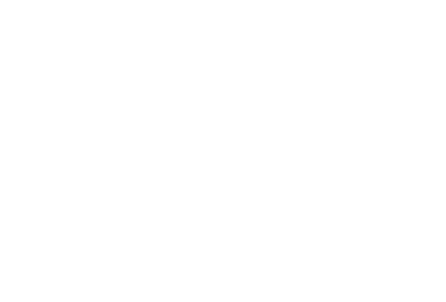
\includegraphics[width=\linewidth]{images/real_data_rm_irf.png} 
    \caption{Monetary policy shock}
    \label{real_rm_irf}
  \end{subfigure}
  %
  \begin{subfigure}{0.8\textwidth}
    \centering  
    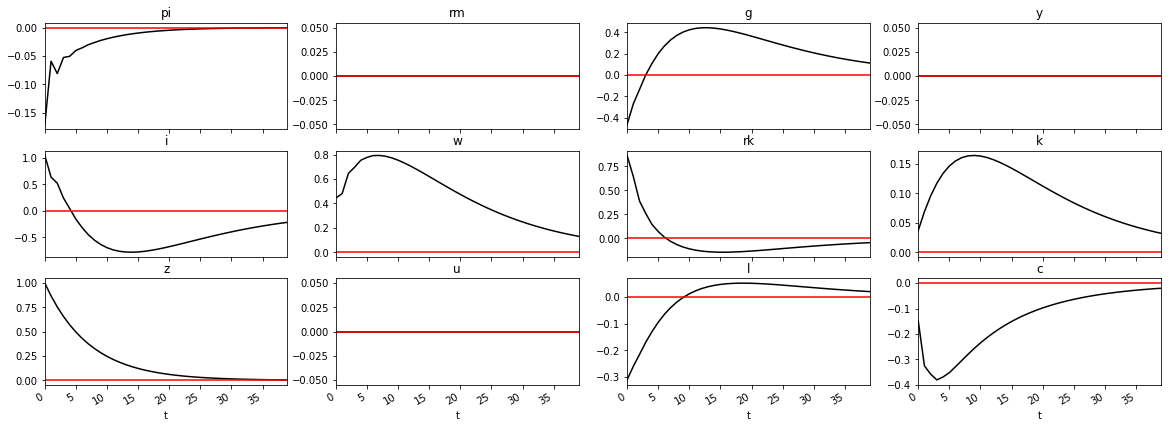
\includegraphics[width=\linewidth]{images/real_data_z_irf.png}
    \caption{Technology shock}
    \label{real_z_irf}
  \end{subfigure}
  %
  \begin{subfigure}{0.8\textwidth}
    \centering  
    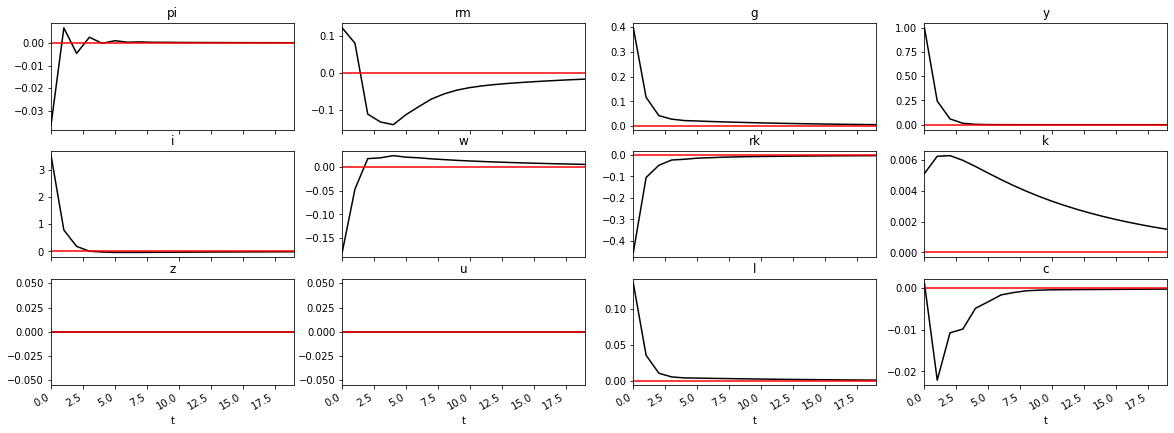
\includegraphics[width=\linewidth]{images/real_data_y_irf.png}
    \caption{Output shock}
    \label{real_y_irf}
  \end{subfigure}
  %
  \begin{subfigure}{0.8\textwidth}
    \centering  
    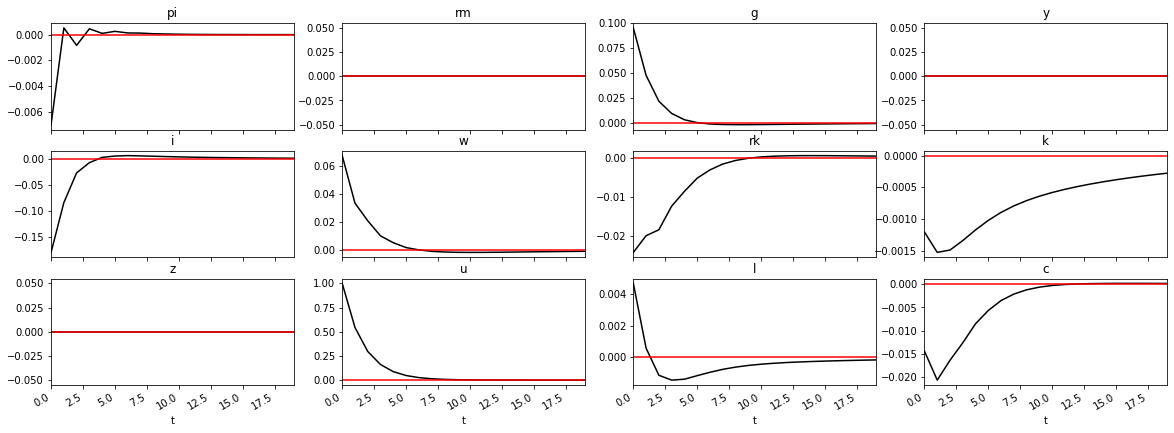
\includegraphics[width=\linewidth]{images/real_data_u_irf.png}
    \caption{Unemployment shock}
    \label{real_u_irf}
  \end{subfigure}

  \caption{IRFs to shocks to each of the exognous states in the model fit to real US macroeconomic data.}
  \label{real_irfs}
\end{figure} 

Figure \ref{real_irfs} shows IRFs for shocks to the 4 exogenous processes in the real US data model.

\section{Discussion and Conclusion}

\newpage
\printbibliography

\newpage
\appendix
\section{Proofs} \label{proofs}

\theoremstyle{definition}
\begin{theorem}
  For a set of variables $\mathbf{w}$ suppose a distribution $f(\mathbf{w})$ is faithful to a DAG $g$ of the type in figure \ref{dsge_dag} for some partition of $\mathbf{w}$ into $\mathbf{z}$, $\mathbf{x}$, and $\mathbf{y}$. Then a log-linearised DSGE model $M$ is faithfully represented by the same DAG if and only if it satisfies (\ref{constraint_test:3}) and (\ref{constraint_test:1}).
\end{theorem}
\begin{proof}
  \textit{Necessary:} The DAG satisfies the conditional independence relationships by construction. \\
  \textit{Sufficient:} Proof by contradiction: \\
  Suppose not. Then $M$ is faithfully represented by a DAH $h$ which is different to $g$. Since $M$ is still a log-linear DSGE solution it must still have a faithful DAG representation of the general form in figure (\ref{dsge_dag}). Therefore, the difference must be that $h$ classifies one or more of the variables in $\mathbf{w}$ differently than $g$. Define the following notation: $g_x$ is the set of variables that are categorised as endogenous states in DAG  $g$ and likewise for $h$ and other categories. \\
  Continue by considering cases: \\
  Case 1: $a \in g_y \text{ and } a \in h_x$ \\
    (\ref{constraint_test:3}) fails because in $g$ $\mathbf{z}_t$ has a direct path to $a$ in $g$. Contradiction. \\
  Case 2: $a \in g_y \text{ and } a \in h_z$ \\
    (\ref{constraint_test:3}) fails because there is a direct path from $\mathbf{x}_t$ to $a$ in $g$. Contradiction. \\
  Case 3: $a \in g_x \text{ and } a \in h_y$ \\
    (\ref{constraint_test:1}) fails because $a$ is not in the conditioning set for this test in $h$ and therefore there is an unblocked backdoor path from $a$ to the other time $t$ endogenous variables in $g$. Contradiction. \\
  Case 4: $a \in g_x \text{ and } a \in h_z$ \\
    (\ref{constraint_test:3}) fails because there is a direct path from $\mathbf{x}_t$ to $a$ in $g$. Contradiction.
  Case 5: $a \in g_z \text{ and } a \in h_y$ \\
    (\ref{constraint_test:1}) fails because there is a direct path from $a$ to any time $t$ endogenous variable in $g$. Contradiction. \\
  Case 6: $a \in g_z \text{ and } a \in h_x$ \\
    (\ref{constraint_test:1}) fails because there is a direct path from $a$ to any time $t$ endogenous variable in $g$. Contradiction. 
\end{proof}

\end{document}
